\section{Development and Training Provenance}\label{app:history}
RQ1 uses the original epoch-28,170 checkpoint; RQ2 also compares the frozen
epoch-34,000 candidate. The monitoring
snapshot below is a separate measurement at epoch 28,159. Historical
single-seed comparisons and compute records are retained here to distinguish
provenance from final performance.
\subsection{Recorded full-scale validation result}\label{sec:full_results}

Table~\ref{tab:full_results} reports the final scheduled monitoring evaluation
recorded for the selected full-scale slot/type run, at epoch 28,159 after
approximately 11.07 billion simulated frames. The separately downloaded
checkpoint is from epoch 28,170. These values are post-correction,
morphology-matched evaluations, not measurements of that later checkpoint
or of the independent test split.

\begin{table}[t]
\centering
\small
\caption{Recorded full-scale monitoring snapshot. Validation contains
1,048 held-out clips; each evaluation uses one selected trained body per clip.
The active resident pool is difficulty-biased. Values are the stored
distributed logging summaries from run \texttt{3mvgad6f}, epoch 28,159;
no confidence intervals or all-shape coverage are implied.}\label{tab:full_results}
\begin{tabular}{lrr}
\toprule
Metric & Hard resident pool & Validation holdout \\
\midrule
Success rate (\%) $\uparrow$ & 89.84 & 98.47 \\
Mean body-position error (m) $\downarrow$ & 0.0960 & 0.0698 \\
Mean global body-rotation error (rad) $\downarrow$ & 0.2261 & 0.1760 \\
Mean maximum-joint position error (m) $\downarrow$ & 0.1848 & 0.1412 \\
Windowed normalized jerk $\downarrow$ & 1,442.8 & 1,151.7 \\
High-jerk windows (\%) $\downarrow$ & 31.05 & 27.25 \\
\bottomrule
\end{tabular}
\end{table}

The validation score is higher than the resident-pool score, while the
reported errors are lower. This comparison is consistent with a curriculum
that concentrates residency on difficult clips: the resident pool is not an
independent uniform sample of the training distribution. Its 89.84\% success
rate should not be interpreted as the success rate of the entire training
corpus, nor should the difference be described as validation outperforming
an IID training sample.

\begin{figure}[t]
\centering
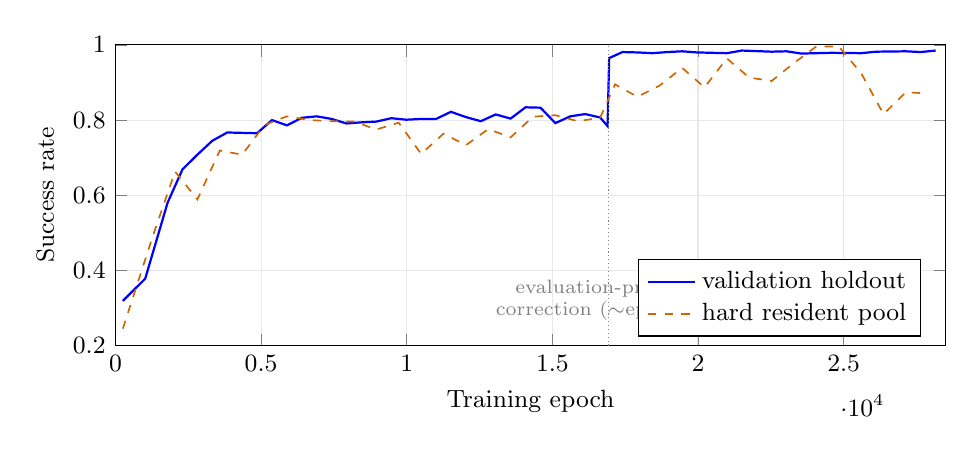
\begin{tikzpicture}
\begin{axis}[
  width=\linewidth, height=5.4cm,
  xlabel={Training epoch}, ylabel={Success rate},
  xmin=0, xmax=28500, ymin=0.2, ymax=1.0,
  legend pos=south east, legend cell align=left, legend style={font=\small},
  tick label style={font=\small}, label style={font=\small},
  grid=both, grid style={gray!18},
]
\addplot[thick, blue] coordinates {
(255,0.319)(1023,0.378)(1791,0.580)(2303,0.669)(2815,0.708)(3327,0.745)
(3839,0.767)(4351,0.766)(4863,0.765)(5375,0.800)(5887,0.786)(6399,0.806)
(6911,0.810)(7423,0.803)(7935,0.791)(8447,0.794)(8959,0.796)(9471,0.805)
(9983,0.801)(10495,0.803)(11007,0.803)(11519,0.822)(12031,0.808)(12543,0.797)
(13055,0.815)(13567,0.804)(14079,0.834)(14591,0.833)(15103,0.792)(15615,0.810)
(16127,0.816)(16639,0.807)(16895,0.784)(16950,0.965)(17407,0.981)(17919,0.980)
(18431,0.978)(18943,0.981)(19455,0.983)(19967,0.980)(20991,0.978)(21503,0.985)
(22527,0.982)(23039,0.983)(23551,0.977)(24575,0.979)(25599,0.978)(26111,0.982)
(27135,0.983)(27647,0.981)(28159,0.985)
};
\addlegendentry{validation holdout}
\addplot[semithick, orange!80!black, dashed] coordinates {
(255,0.245)(1279,0.490)(2047,0.663)(2815,0.589)(3583,0.719)(4351,0.708)
(5119,0.787)(5887,0.810)(6655,0.800)(7423,0.797)(8191,0.796)(8959,0.775)
(9727,0.793)(10495,0.710)(11263,0.764)(12031,0.733)(12799,0.776)(13567,0.754)
(14335,0.809)(15103,0.813)(15871,0.797)(16639,0.806)(17151,0.895)(17919,0.862)
(18687,0.892)(19455,0.939)(20223,0.887)(20991,0.964)(21759,0.913)(22527,0.904)
(23295,0.952)(24063,0.996)(24831,0.996)(25599,0.925)(26367,0.816)(27135,0.874)
(27903,0.871)
};
\addlegendentry{hard resident pool}
\draw[gray, densely dotted] (axis cs:16920,0.2) -- (axis cs:16920,1.0);
\node[anchor=south, font=\scriptsize, gray, align=center]
  at (axis cs:16920,0.24) {evaluation-protocol\\correction ($\sim$ep.\ 16.9k)};
\end{axis}
\end{tikzpicture}
\caption{Scheduled success rate over training for the full-scale slot/type
run (\texttt{3mvgad6f}). The step near epoch 16.9k is the morphology-matched
evaluation correction plus its sampling change, not an instantaneous learning
event; pre-correction points use the earlier, sometimes mismatched
reference-to-asset assignment and are not comparable to the post-correction
curve. After the correction the holdout success rate climbs from about
0.96 to a stable 0.98--0.985. The resident-pool curve is noisier because
residency is continually re-concentrated on hard clips.}\label{fig:learning_curve}
\end{figure}

The 98.47\% result supports strong tracking of the selected held-out
clip/body pairs under the specified threshold. It does not establish
all-body success for those clips, unseen-body generalization, or an untouched
test-set score. The thresholded success rate is complemented by position,
rotation, and smoothness measures because a successful rollout can still
have visible local errors or jitter.

% Evidence: note/README.note.md, section 76, recorded 2026-09-07.
% Do not replace the monitoring epoch with last.ckpt's epoch.
The run record is available at
\href{https://wandb.ai/yugoamaryl/hhi-protomotions/runs/3mvgad6f}
{the full-scale W\&B run}. The current table uses the recorded snapshot,
not a newly executed evaluation.


\subsection{Historical single-seed reference grid}
Cases A--D use refined references and E--H use unrefined references.
Within-run variation must not be interpreted as uncertainty across training
runs. The main architecture conclusion uses repeated refined runs instead.
\begin{table}[t]
\centering
\small
\caption{Historical seed-0 development grid. Success uncertainty is variation across eight evaluations within each run. Other columns are their means. Refined and unrefined policies track different targets. The three-seed comparison is in Table~\ref{tab:architecture_seeds}.}\label{tab:ablation_results}
\begin{tabularx}{\linewidth}{@{}llYrrrr@{}}
\toprule
Case & Architecture / data & Success (\%) & gt err & gr err & Jerk & HJ\% \\
\midrule
A & temporal MLP, refined        & 97.5 $\pm$ 0.8 & 0.109 & 0.207 & 1{,}729 & 33.3 \\
B & attention, refined           & 97.5 $\pm$ 1.4 & 0.098 & 0.228 & 3{,}455 & 40.4 \\
C & slot/type, refined           & \textbf{98.1 $\pm$ 0.6} & 0.097 & 0.226 & \textbf{1{,}757} & 34.2 \\
D & slot/type + AdaLN, refined   & 97.1 $\pm$ 1.2 & \textbf{0.090} & 0.220 & 3{,}145 & 38.9 \\
E & slot/type, unrefined         & 97.9 $\pm$ 0.6 & 0.102 & 0.219 & 1{,}422 & 29.6 \\
F & temporal MLP, unrefined      & 96.2 $\pm$ 1.6 & 0.115 & 0.212 & 2{,}927 & 36.6 \\
G & attention, unrefined         & 97.8 $\pm$ 1.2 & 0.098 & 0.219 & 3{,}117 & 34.9 \\
H & slot/type + AdaLN, unrefined & 97.5 $\pm$ 0.9 & 0.091 & 0.207 & 2{,}956 & 34.0 \\
\bottomrule
\end{tabularx}
\end{table}
\subsection{Compute accounting}
We retain W\&B logs, resolved configurations, checkpoint epochs, and local
results for compute accounting. Small-scale development and full-scale
training costs should be reported separately, including resumed segments and
failed launches when discussing practical cost. GPU-hours, rather than
epoch counts alone, quantify this budget.

Table~\ref{tab:compute_accounting} reports parameter counts and single-A40
wall-clock cost for the eight corrected 150-clip runs, all completed at the
6,000-epoch budget. Parameter counts are computed analytically from
each run's resolved model configuration (encoder, transformer or flat-MLP,
and head widths), not read from a stored checkpoint file, since every linear
layer in this codebase is instantiated with \texttt{nn.LazyLinear} and has no
fixed parameter count outside a materialized model. Parameter count is set by
the architecture only, so the refined/unrefined pairs share a count
(A/F, B/G, C/E, D/H).

\begin{table}[t]
\centering
\small
\caption{Parameter counts and single-GPU wall-clock cost for the eight
corrected 150-clip runs (seed 0, one A40 each, 6,000 epochs). Actor and
critic are separate networks with independent parameters.}\label{tab:compute_accounting}
\begin{tabularx}{\linewidth}{@{}llrrrY@{}}
\toprule
Case & Arch & Actor params & Critic params & Total params & GPU-h \\
\midrule
A / F & temporal MLP        & 57,349,557 & 8,524,801 & 65,874,358 & 15.8 / 14.4 \\
B / G & attention           & 45,430,197 & 5,800,705 & 51,230,902 & 23.5 / 21.5 \\
C / E & slot/type           & 45,434,037 & 5,804,545 & 51,238,582 & 23.7 / 23.9 \\
D / H & slot/type + adaLN   & 46,256,053 & 5,804,545 & 52,060,598 & 23.9 / 22.4 \\
\bottomrule
\end{tabularx}
\end{table}

Two consequences run against a naive intuition. First, the temporal MLP has
the most total parameters of any architecture, not the fewest: its actor's
first layer reads the full raw concatenation of every observation category
(5,248 dimensions) directly, which alone costs more parameters than the
attention models' three token encoders and transformer combined. The
attention models compress that same information to a 256-dimensional token
per source before the shared final head, trading parameters for the added
transformer computation. Second, despite having more parameters, the temporal
MLP is the fastest to train by a wide margin (15.8/14.4 vs.\ 21.5--23.9
GPU-hours) -- parameter count does not predict wall-clock cost here, since the
attention models pay for multiple sequential module calls (three encoders,
then a transformer stack) rather than one large matrix multiplication chain.
Actor-only adaLN-Zero adds a small but non-negligible cost over slot/type
(roughly 822,000 actor parameters from the per-layer modulation networks and
morphology encoder), a capacity difference rather than evidence of a smoothness benefit.

The full-scale selected run shares C and E's architecture exactly (same
encoder, transformer, and head widths;
\texttt{mlp\_wide\_stage2\_discover\_attention\_slot\_type.py} inherits
these constants unchanged from the 150-clip experiment file), so its
parameter count is also 51,238,582. It ran on six A40 GPUs
(\texttt{ddp}, 32-bit, 2,048 environments and an 8,192 minibatch per GPU) for
roughly 28,170 epochs. The logged rank-0 wall time is about 77\,h, of which
one interruption near epoch 760 accounts for about 3\,h, giving on the order
of 450 GPU-hours; the run is not directly comparable to the eight matched
single-GPU development runs. An early restart after a memory-related failure
resumed from the last checkpoint with the resident pool reduced from 256 to
128 clips per rank and the local cache multiplier set to 1.0; because
configs are reloaded from the pickle on resume, the frozen configuration
still records the pre-restart pool size of 256. The earlier failed launch was
logged into the same run and is not separately quantifiable.
Segment-level cost accounting remains incomplete. Approximate full-scale
GPU-hours cannot establish superior compute efficiency against the smaller
matched development runs.
